%
% File finalreport.tex
%
%% Based on the style files for ACL 2018 and NAACL 2018, which were
%% Based on the style files for ACL-2015, with some improvements
%%  taken from the NAACL-2016 style
%% Based on the style files for ACL-2014, which were, in turn,
%% based on ACL-2013, ACL-2012, ACL-2011, ACL-2010, ACL-IJCNLP-2009,
%% EACL-2009, IJCNLP-2008...
%% Based on the style files for EACL 2006 by 
%%e.agirre@ehu.es or Sergi.Balari@uab.es
%% and that of ACL 08 by Joakim Nivre and Noah Smith

\documentclass[11pt,a4paper]{article}
\usepackage[hyperref]{naaclhlt2019}
\usepackage{times}
\usepackage{latexsym}
\usepackage{graphicx}
\usepackage{multirow}

\usepackage{url}

\aclfinalcopy % Uncomment this line for the final submission
%\def\aclpaperid{***} %  Enter the acl Paper ID here

%\setlength\titlebox{5cm}
% You can expand the titlebox if you need extra space
% to show all the authors. Please do not make the titlebox
% smaller than 5cm (the original size); we will check this
% in the camera-ready version and ask you to change it back.

\newcommand\BibTeX{B{\sc ib}\TeX}

\title{Prediction of Europe Football Outcomes using Deep Networks}

\author{Kornraphop Kawintiranon \\
  Department of Computer Science \\
  Georgetown University \\
  Washington, DC, USA \\
  {\tt kornraphop.k@cs.georgetown.edu} \And
  Hanjing Wang \\
  Department of Analytics \\
  Georgetown University \\
  Washington, DC, USA \\
  {\tt hj@georgetown.edu}\\\AND
  Armaan Khullar \\
  Department of Computer Science \\
  Georgetown University \\
  Washington, DC, USA \\
  {\tt ak1643@georgetown.edu} \And
  Jiajia Liu \\
  Department of Analytics \\
  Georgetown University \\
  Washington, DC, USA \\
  {\tt jl2292@georgetown.edu} \\}

\date{}

\begin{document}
\maketitle
\begin{abstract}
Obtaining the performances and results of Europe Football teams such as Barcelona, Real Madrid, Bayern Munich, etc is one of the popular questions in the sports field. For most soccer statistics, the observations are very limited to aggregated data such as goals, shots, and fouls. However, a football game could generate many more events, and it is very important and interesting to take into account the context in which those events are generated. This dataset is a result of web scraping and integrating different data sources. The central element is the text commentary. All the information is extracted from the event descriptions. Our work involves three models: Artificial Neural Networks (ANN), Convolutional Neural Networks (CNN), and Recurrent Neural Networks (RNN). The ANN achieves approximately 66\% of accuracy on our validation set for football outcome prediction. The CNN utilizes only textual features, and its performance using text alone is approximately 66\% of accuracy on the validation set for outcome prediction. The RNN is established with an accuracy of 96\% for predicting the event sequences. Finally, we design an ensemble ANN model in which we combine the results from separate models to achieve a better performance. We aim to investigate outcomes of European Football teams and improve the prediction results.
\end{abstract}


\section{Introduction}

Soccer is arguably the most popular sport in the world. 3.5 billion people, nearly half of the world’s population, watched the World Cup this past year alone.  It only necessitates a ball and an open space, which allows anyone, regardless of background, to participate. Given that soccer is such a closely followed sport, enthusiasts, gambling companies, and financial institutions, are forever seeking ways of predicting which team will win a match or tournament.

In this paper, we will propose methodologies and empirical results to help better with these predictions. We limit our study to European soccer and to the five largest European soccer leagues: England, Spain, Germany, Italy, and France, between 2011 and 2017. In our experiments, we implemented deep learning models to analyze both team-based and game-based data. During our experimentation, we found some interesting questions that we sought to answer:

1: What are the top teams based on their goals of performance?
2: Can we predict the sequence of the events that would transpire during a game’s second half?
3: Can we use commentary during a game’s first half to predict the final outcome of the game?

We will first discuss the related work before going into the details of our feature engineering techniques, experiments, and results.


\section{Related Work}

The majority of research on this task has been done on behalf of researchers at private organizations or by freelancers. Publicly available work in this area is, therefore, limited. However, we found papers related to predicting soccer match results in the english premier league~\cite{soccerpredict,timmaraju2013game,joseph2006predicting,rue2000prediction} , which was written by students at Stanford. In their research, the authors focus on soccer matches in the English Premier League. They use a variety of machine learning models such as neural networks, naive bayes, hidden markov models, and support vector machines. For each of their models, they run a three-classification problem in which they try to predict whether a game ends in a win, loss, or a tie, from the host team’s perspective. The paper has nice results, but the authors are only using considering one league, and have a dataset with different features than what we have available. Nonetheless, we borrowed some ideas such as constructing a three-class classification problem for some of our own models. Finally, we were also influenced by the work Matheus Gonzaga and Alexandra Rodriguez from their blog We used Neural Networks to predict the 2018 World Cup champion~\cite{worldcup}, on the website Poatek. In particular, they used a Recurrent Neural Network in order to predict the winner of the 2018 World Cup. Although our particular problem and the data set are different, these two papers served as a reference of ideas to expand on


\section{Datasets}

For this project, we are focusing on the “events.csv” Football Events dataset that was provided by Kaggle. This dataset contains event data for 9,074 games for the top five European soccer leagues: England, Spain, Germany, Italy, and France, between 2011 and 2017.  It records information pertaining to 16 types of events that transpired over the course of a game. If one of these events takes place during a game, the minute and the type of event are stored in a row, along with text commentary and information about the players involved and the teams they belonged to. There were other granular details, like “body part”, which we considered as inconsequential and thus ignored in during our feature selection. There can be multiple events that happen even in the same minute.


\section{Methodologies}

\begin{figure*}
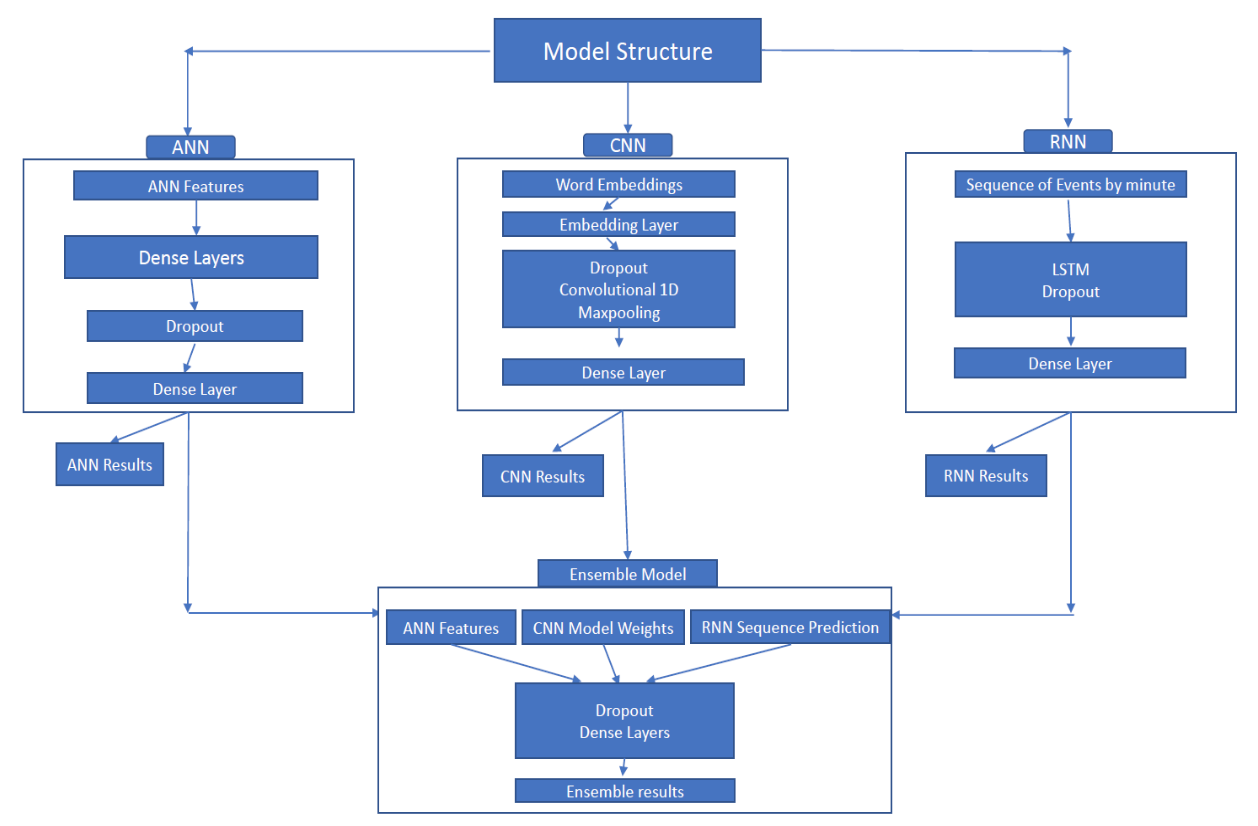
\includegraphics[width=\textwidth]{./img/fig-1.png}
\caption{\label{model-figure} Deep networks architecture.}
\end{figure*}

\subsection{Artificial Neural Networks (ANN)}

The first experiment we constructed was a three-classification problem in which we tried to predict whether the home team wins, the away team wins, or the game ends in a tie. This involved feature engineering of the original data in which we create both game-based and team-based features. We first generate 38 game-based features in which for each game and team, we extract the number of goals, fouls, red cards, yellow card, and the other events. The team-based data with 10 features are generated in which the average goals and the winning percentage for each team are also considered. The model has a total of 48 features for predicting the outcomes of more than 9000 games. After feature preparation, our ANN model is established for this classification problem. We train three different models, each over 80 minutes, 70 minutes, 60 minutes, and 45 minutes, respectively. The models have several dense layers with 64 neurons and a rectifier activation function for each layer. We also added dropout regularization to reduce the overfitting problem.

\subsection{Convolutional Neural Networks (CNN)}

In this model, we aggregate the comments from commentators of all events that occurred during the first half of each game in order to predict the team that will win the game. We have tried word2vec~\cite{mikolov2013efficient} but model accuracy was too low, therefore, word embeddings were built based on all the game’s comments and feed them into the CNN model. This model is a three-classification problem as before. The result of each game is a probability of the home team winning, the away team winning, or the game ending in a tie.

\subsection{Recurrent Neural Networks (RNN)}

In this model, we try to predict the sequence of events that will transpire during the second half of a soccer game using information from the first half~\cite{sutskever2014sequence}. In particular, for each game we look at the first 45 minutes. Each of those minutes in turn consists of a sequence of binary events, such as whether a goal was scored, a foul was committed, a red card given, etc. In this experiment, we create a Long short-term memory (LSTM) model to predict a game’s sequence of events for each minute of the second half using the sequence of events from the first half. We initially try to predict whether each of the events occur for each minute of a game, regardless of the team involved. We then double our original event features by creating a separate event attribute dedicated to each team. We also add in other features such as “assist method” and “fast break”. We train our model and predict the sequence of events for each minute of the second half for each game.

\subsection{Ensemble Model: Combining all models}

The final experiment is to combine the separate models by adding the new features generated in CNN and LSTM model to the original ANN three-classification model. We use the CNN model’s weights and event sequence prediction results from the LSTM as the additional features. In particular, we use the predicted results of the LSTM model that separate features for each team. We thus have 343 features in the final ANN model.


\section{Results}

From Table~\ref{seq-result-table}, the LSTM models achieve good performances. Therefore, by after adding the RNN features to the ANN model, we could get higher accuracy for the ensemble model compared to the CNN model. Moreover, better results could be obtained if we make predictions only for the top teams as shown in Figure~\ref{acc-figure}.

The less teams we predict, the better results we could get. From figure below, we also make experiments for different time periods as demonstrated in Figure~\ref{min-acc-figure}. If we use the event information of a longer time period, we could get more accurate predictions.

\begin{table}[h!]
\begin{center}
\resizebox{\columnwidth}{!}{\begin{tabular}{|c|c|c|}
\hline
{Model} & \bf Evaluation & \bf Accuracy \\\hline
LSTM (w/o team info) & Random 33\% & 0.9286 \\
\hline
LSTM (with team info) & Random 33\% & 0.9630 \\
\hline
\end{tabular}}
\end{center}
\caption{\label{seq-result-table} Sequence of Events Prediction. }
\end{table}

\begin{figure}
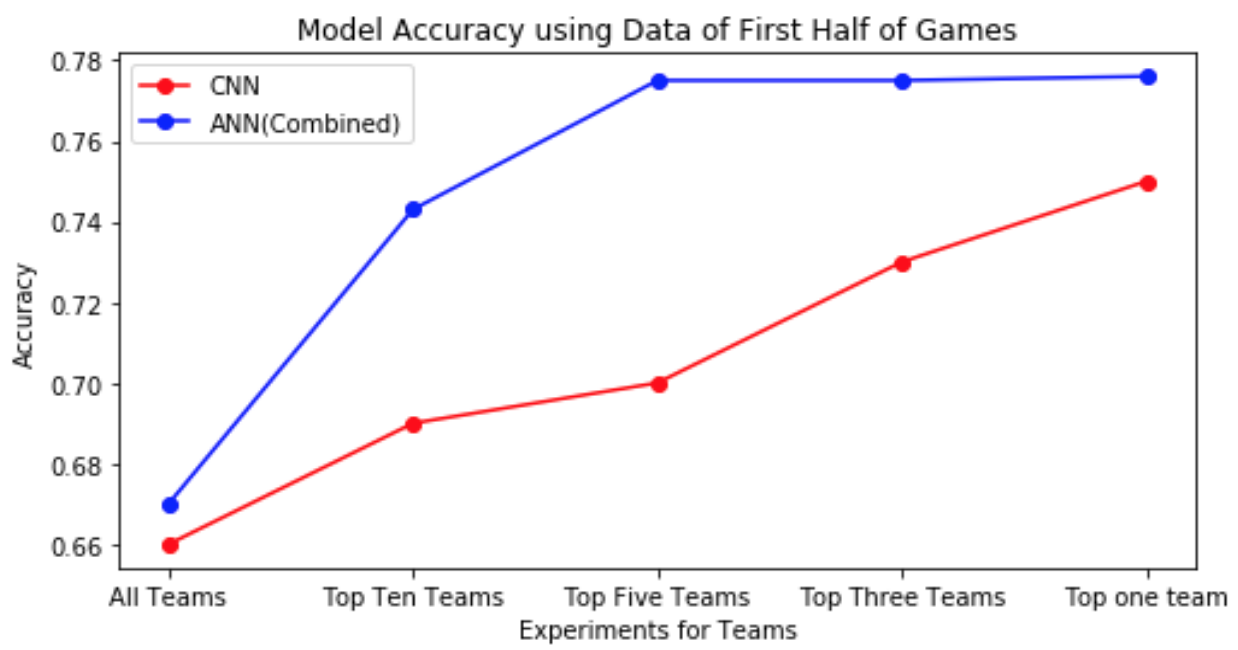
\includegraphics[width=\columnwidth]{./img/fig-2.png}
\caption{\label{acc-figure} Model Accuracy using Data of First Half of Games.}
\end{figure}

\begin{figure}
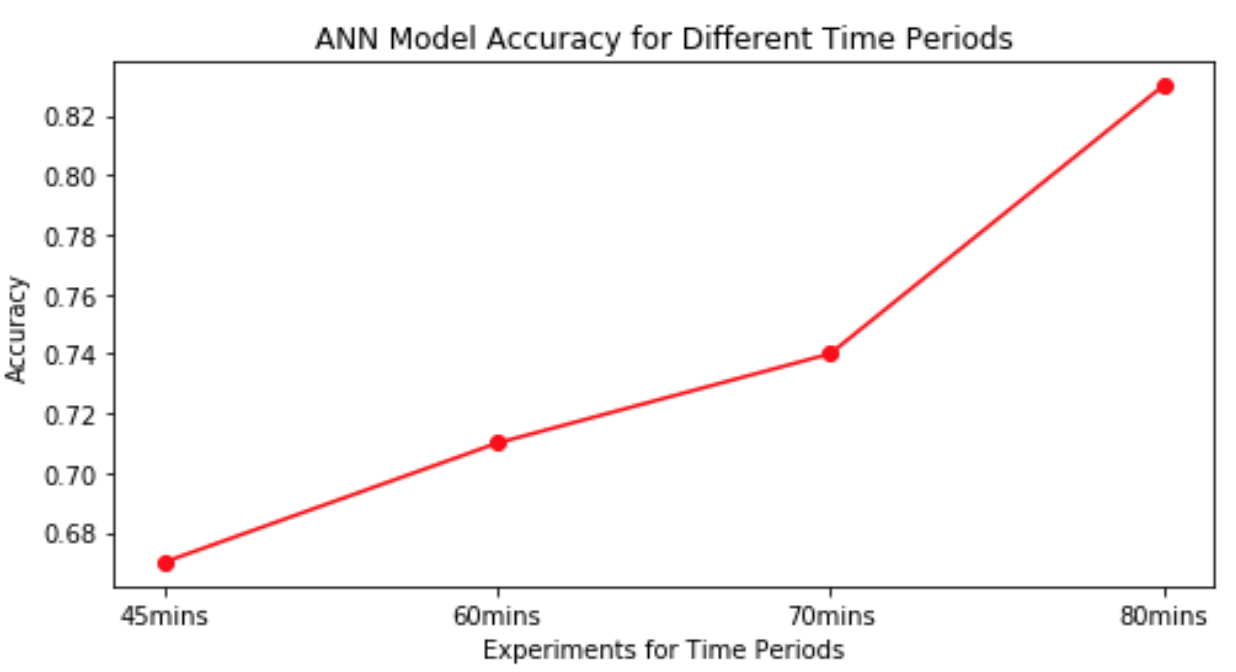
\includegraphics[width=\columnwidth]{./img/fig-3.png}
\caption{\label{min-acc-figure} Ensembled Model Accuracy for Different Time Periods.}
\end{figure}


\section{Conclusions}

Overall, it seems that we have very interesting results and observations. We utilize textual comments from commentators during the first half of each game, in order to predict the outcome of a game (win-loss-tie). First, we use only the textual data with the CNN to perform the predictions. The model accuracy is only 66\% with a randomized validation set, but we can improve the model performance by extracting textual comments into event features. Furthermore, preliminary results suggest that the ANN model performs better if we consider more minutes per game. For example, we see that we get a higher accuracy for an ANN that is trained over 80 minutes, followed by 70 minutes, 60 minutes, and 45 minutes. While our LSTM models are able to achieve a high accuracy, it is difficult to get a probability that is greater than 50\% for any given event in any minute of the second half. Thus, we are unable to convert the probabilities into binary values without them all being 0. Nonetheless, the LSTM models do provide information - probabilities - which we can nonetheless use. When we combine the game-based and team-based features of the ANN, with the predictions generated by the CNN and the LSTM, we create our ensemble model. We see that it performs better if we consider only the top teams. The best accuracy is up to 78\% if we use this ensemble model to predict the best win-rate team - Barcelona.

\bibliography{finalreport}
\bibliographystyle{acl_natbib}


\end{document}
